\documentclass[journal,12pt,onecolumn]{IEEEtran}
\usepackage{listings}
\usepackage{ragged2e}
\usepackage[utf8]{inputenc}
\usepackage{subcaption}
\usepackage{tikz}
\usepackage[export]{adjustbox}
\usepackage{tkz-euclide} % loads  TikZ and tkz-base
\usetkzobj{all}
\usetikzlibrary{calc,math}
\usepackage{amsmath}
\title{Document on Question 28 Exercise(8.1)}
\author{Pothukuchi Siddhartha}

\begin{document}

\maketitle
\begin{abstract}
This a simple document explaining a question about the concept of similar triangles.
\end{abstract}
Download all python codes from 
%
\begin{lstlisting}[frame= single]
svn co https://github.com/SiddharthPh/Summer2020/trunk/document/codes
\end{lstlisting}
%
\section*{\textbf{Question}}
In right triangle ABC, right angled at C, M is
the mid-point of hypotenuse AB. C is joined to
M and produced to a point D such that DM =
CM. Point D is joined to point B. Show that:
\newline
a)$\triangle  AMC  \cong   \triangle  BMD $
\newline
b)$\triangle DBC $ is a right angle.
\newline
c)$\triangle  DBC  \cong  \triangle  ABC $
\newline
d)CM = $\frac{1}{2}$ AB

\section*{\textbf{Solution}}
The python code for the figure is
\begin{lstlisting}[frame=single]
./code/traingle.py
\end{lstlisting}
The latex- tikz code is
\begin{lstlisting}[frame=single]
./figs/triangle.tex
\end{lstlisting}
The above latex code can be compiled as standalone document
\begin{lstlisting} [frame=single]
./figs/triangle_fig.tex
\end{lstlisting}
\begin{figure}[h]
\begin{subfigure}{0.5\textwidth}
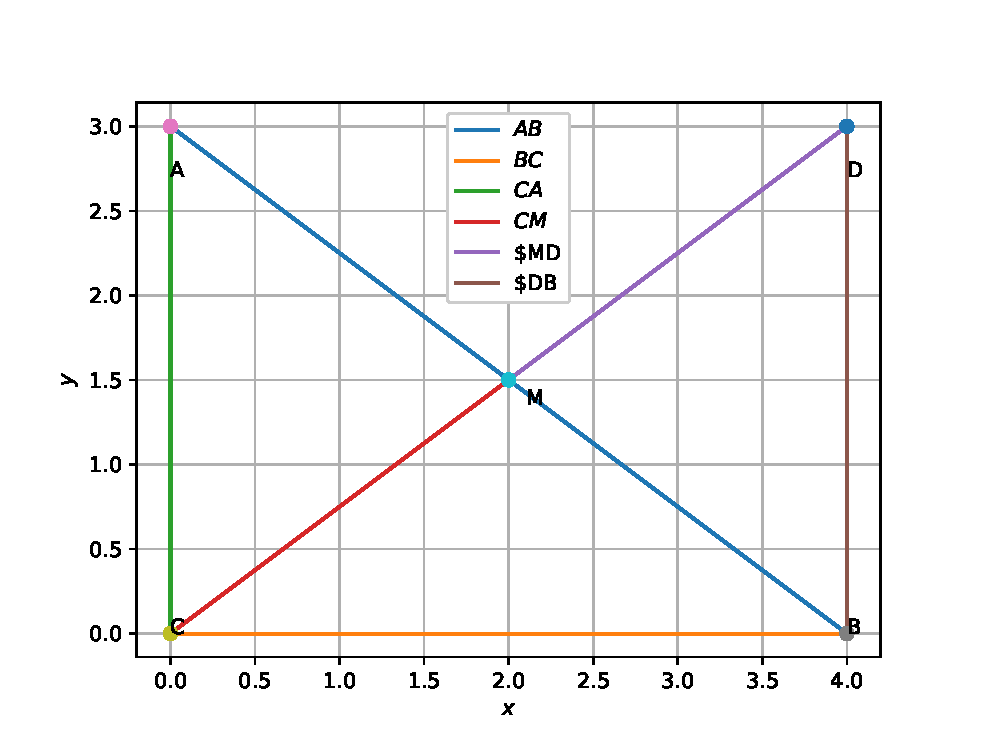
\includegraphics[width=0.9\linewidth, height=5cm]{./figs/triangle.eps}
\caption{By Python}
\end{subfigure}
%
\begin{subfigure}{0.4\textwidth}
\begin{flushright}


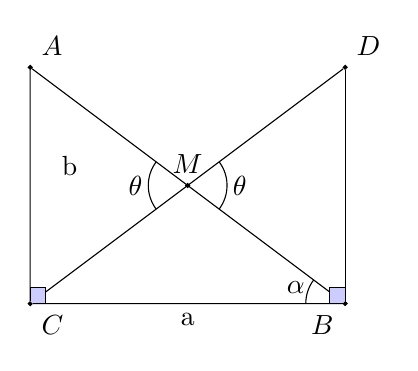
\begin{tikzpicture}
[scale=1,>=stealth,point/.style={draw,circle,fill = black,inner sep=0.5pt},]

%Triangle sides
\def\a{4}
\def\b{3}
\def\c{sqrt(\a^2+\c^2)}



%Labeling points
\node (A) at (0,\b)[point,label=above right:$A$] {};
\node (B) at (\a, 0)[point,label=below left:$B$] {};
\node (C) at (0, 0)[point,label=below right:$C$] {};
\node (M) at (\a*0.5,\b*0.5)[point,label=above:$M$] {};
\node (D) at (\a,\b)[point,label=above right:$D$] {};


%Drawing triangle ABC
\draw (A) -- node[left] {$\textrm{}$} (B) -- node[below] {$\textrm{a}$} (C) -- node[above,xshift=5mm] {$\textrm{b}$} (A);

%Joining CD
\draw (C)--(D);
%Joining BD
\draw (B)--(D);

%Drawing and marking angles
\tkzMarkAngle[fill=orange!40,size=0.5cm,mark=](A,M,C)
\tkzMarkAngle[fill=orange!40,size=0.5cm,mark=](B,M,D)
\tkzMarkAngle[fill=green!40,size=0.5cm,mark=](A,B,C)
\tkzMarkRightAngle[fill=blue!20,size=.2](A,C,B)
\tkzMarkRightAngle[fill=blue!20,size=.2](D,B,C)
\tkzLabelAngle[pos=0.65](A,M,C){$\theta$}
\tkzLabelAngle[pos=0.65](B,M,D){$\theta$}
\tkzLabelAngle[pos=0.65](A,B,C){$\alpha$}


\end{tikzpicture}

\caption{By Latex-tikz}
\end{flushright}
\end{subfigure}
\caption{Obtained by executing the  above codes.}
\end{figure}
%
\subsection*{\textbf{Sol.a)}}
\begin{flushleft}
From the above figure,
$$
C=
\begin{pmatrix}
0\\
0
\end{pmatrix}
,A=
\begin{pmatrix}
0\\
b
\end{pmatrix}
,B=
\begin{pmatrix}
a\\
0
\end{pmatrix}
$$
As, M is the midpoint of AB
$$
M=
\begin{pmatrix}
a/2 \\
b/2 
\end{pmatrix}
$$
Therefore Coordinates of D are
$$
D=
\begin{pmatrix}
a\\
b
\end{pmatrix}
$$
\newline
\newline
$\triangle AMC$ and $\triangle DMB$ are congruent to each other by SAS congruency.
\newline
(i) Side AM  is equal to the corresponding side BM  [As M is midpoint of AB]
\newline
(ii)Side CM of is equal to corresponding side DM [As M is midpoint of DC]
\newline
(iii)$\angle AMC$ = $\angle DMB$ [ Vertically Opposite Angles]
\end{flushleft}
\subsection*{\textbf{Sol.b)}}
\begin{flushleft}

In $\triangle ACB$ 
\newline
$(AB)^2=a^2+b^2$   Since $\angle ACB$ = 90$^{\circ}$[ Pythagorus theorem]
\newline
\newline
In $\triangle DBC$  [DB = D-B = b]  
\newline
\newline
$cos \angle DBC = [((a^2+b^2-(DC)^2)/2ab)]$ 
\newline
\newline
By using distance formula i.e $\sqrt{(x1-x2)^2+(y1-y1)^2}$ we get that AB=DC from the given coordinates.
\newline
$cos\angle DBC = [((a^2+b^2-(AB)^2)/2ab)]$
\newline
$cos\angle DBC=0$
\newline
Therefore, $\angle DBC$ is right angle
\end{flushleft}
\subsection*{\textbf{Sol.c)}}
\begin{flushleft}
$\triangle ACB$ and $\triangle DCB$ are congruent to each other in SAS congruency.
(i)Both the triangles have a common base , a.
\newline
(ii)AC = DB by using distance formula
\newline
(iii)$\angle ACB$ = $\angle DBC$ = 90$^{\circ}$ [ From Solution b]
\end{flushleft}
\subsection*{\textbf{Sol.d)}}
\begin{flushleft}
Since M is the midpoint of CD
\newline
CM=$\frac{1}{2}$ DC
From Solution b) it is clear that DC=AB
\newline
Therefore CM=$\frac{1}{2}$AB
\newline
Hence Proved.

\end{flushleft}
\end{document}
